% chap2.tex
\part{유지보수 및 신기술 적용}
\label{part:module}

% ---------------------------------------------------------------------------- %
%                                  NEW SECTION                                 %
% ---------------------------------------------------------------------------- %

\chapter{pyGRsim 모듈}

\section{개발 원칙, 철학, 구조}

\subsection{철학}
음.. PEP8 따른다? 뭘 써야할지 고민 필요. 철학까지는 없는듯.

\subsection{전체 구조}
pyGRsim 밑에 core 있고 dragon 있고... core와 dragon은 동일한 하위폴더로 분류되어있고..

\subsection{환경 및 의존성}
이것도 위에서 몇 번 언급한 것 같은데 한 곳에서 통일할 필요가 있을듯.

% ---------------------------------------------------------------------------- %
%                                  NEW SECTION                                 %
% ---------------------------------------------------------------------------- %


\section{활용법}
python 레벨에서 이 모듈을 활용하려면 일단 GreenRetrofitModel을 직접 구축하는 예시부터 참고하면 됨.

% ---------------------------------------------------------------------------- %
%                                  NEW SECTION                                 %
% ---------------------------------------------------------------------------- %

\section{pyGRsim 구조별 상세}
pyGRsim이랑 dragon이랑 launcher랑 나누어서 서술할 것임.

\subsection{pyGRsim}
\subsubsection{construction}
구조임
\subsubsection{profile}
프로필임
\subsubsection{hvac}
시스템임
\subsubsection{shape}
모양?임
\subsubsection{model}
모델임

\subsection{dragon}
\subsubsection{construction}
구조임
\subsubsection{profile}
프로필임
\subsubsection{hvac}
시스템임
\subsubsection{shape}
모양?임
\subsubsection{model}
모델임
\subsection{imugi}
eppy 대신하는 좋은 모듈임. 이런저러한 기능을 지원함. 여기서는 뭐뭐뭐 위주로 사용됨. 
\subsection{launcher}
EP 실행하는 모듈임. 모듈 구조는 아래와 같이 되어 있고, 향후 무슨무슨 실행을 고려할 수 있도록 구조화되었음. EP run 도는 부분까지 호출되는 순서는 유의 바람.
EP 돌아가는거 파싱하는 부분도 있음. 이런 가정 하에서 파싱하는거라서 혹시 이게 안되면 잘 안될지도 모름.

% ---------------------------------------------------------------------------- %
%                                  NEW SECTION                                 %
% ---------------------------------------------------------------------------- %

\section{데이터 변환의 구현}
\subsection{grexcel to grjson}
불러올 때 column들 filtering해서 들어오고 ID 붙이고...

\subsection{grjson to GreenRetrofitModel}
일단 reference하는 객체들이 있으니까 만들어놓고 dict에 저장하는 식으로 구현함. surface같은건 마지막에 ref관계 연결해줌. ref를 포함하는 얘들은 나중에 만드는 식으로 하고 fromjson함수에 그 dict들을 추가로 입력으로 받도록 해서 구현함

\subsection{GreenRetrofitModel to EnergyModel}
모든 GRM 객체는 to\_dragon을 가지고 있음 (zone 빼고). 그걸 가지고 하나씩 변환한다고 생각하면 됨. 일단 surface부터 만들어놓고 형상만들고 거기다가 설비를 갖다붙이는 순서로 만듬. 형상만들때 주의해야 하는게 아래 순서로 작업하는 걸 기억해야 함. 그리고 원본 훼손 안되게 해야 하니까 unknown인 얘들은 다시 복원해야 함.

\subsection{EnergyModel to idf}

\subsubsection{idf 기본 설정}
기본적으로 돌아가게 하기 위해서 아래 얘들을 먼저 만들어줘야 함.
\paragraph{Building} 이건 필요함
\paragraph{SimulationOptions} 이것도 필요함

시뮬레이션 똑바로 돌아가려면 또 설정할 것들이 있음.
\paragraph{something} 을 설정해줘야함
\paragraph{something} 을 설정해줘야함
\paragraph{something} 을 설정해줘야함

\subsubsection{DB류 객체들 내보내기}
material, construction, profile 이런 것들은 미리 다 쌓아둔다.

\subsubsection{실재하는 객체들 하나씩 내보내기}
zone, surface, 설비같은 것들에 해당. 모든 EnergyModel 객체들은 다 to\_idf\_object 객체 가지고 있음. 기본적으로는 자기자신을 idfobject화 해서 계속 append하는 건데, 어떤 얘들은 좀 연동이 있어서 이걸 고려해야 함.

\subsubsection{후처리}
할 것들이 좀 있음

\subsubsection{ouptut 관리 등}
결과물 출력할 수 있게 작업해야 함

% ---------------------------------------------------------------------------- %
%                                  NEW SECTION                                 %
% ---------------------------------------------------------------------------- %

\section{EnergyPlus의 실행}
외부에서 입력이 들어오면, 그림 \ref{fig:eplaunchbycode}\와 같이 EnergyPlus가 호출됨
\begin{defaultfigure}
  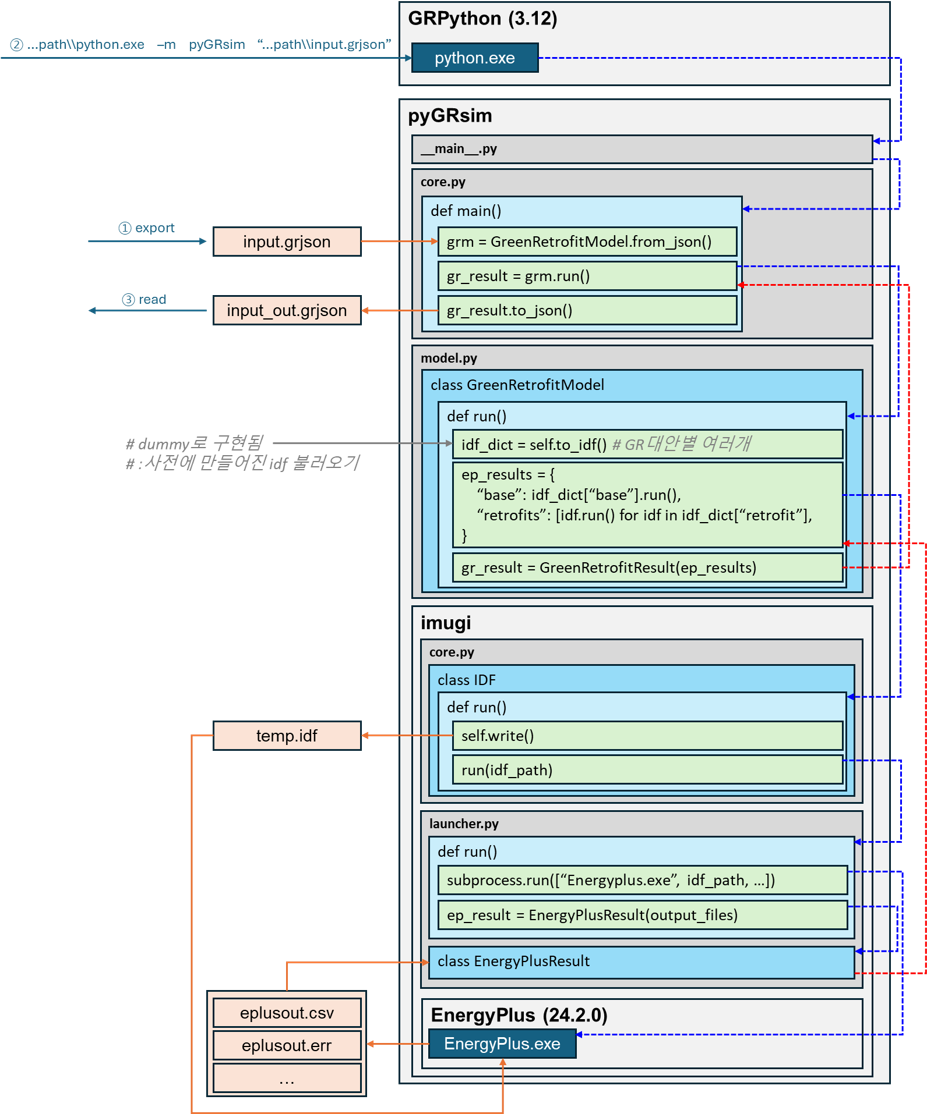
\includegraphics[height=0.99\textheight, width=\textwidth, keepaspectratio]{실행구조도.png}
  \caption{외부 호출 시 EnergyPlus launch되는 호출 흐름}
  \label{fig:eplaunchbycode}
\end{defaultfigure}

% ---------------------------------------------------------------------------- %
%                                  NEW SECTION                                 %
% ---------------------------------------------------------------------------- %

\section{예시코드}

import pyGRsim

% ---------------------------------------------------------------------------- %
%                                  NEW SECTION                                 %
% ---------------------------------------------------------------------------- %

\chapter{알고리즘의 수정과 코드의 유지보수}

\section{알고리즘의 수정 제안}

이런 값들을 바꿔보면서 수정하면 됨

% ---------------------------------------------------------------------------- %
%                                  NEW SECTION                                 %
% ---------------------------------------------------------------------------- %

\section{기본값 변경}

to\_idf\_object 열심히 건들면 됨

% ---------------------------------------------------------------------------- %
%                                  NEW SECTION                                 %
% ---------------------------------------------------------------------------- %

\section{일반적인 코드의 유지보수}

화이팅

% ---------------------------------------------------------------------------- %
%                                  NEW SECTION                                 %
% ---------------------------------------------------------------------------- %

\chapter{신기술 적용}

\section{신기술의 시뮬레이터 적용하기 위해 필요한 개념적인 과정}

지금 체계에 맞아야 함. 예를 들어서,

% ---------------------------------------------------------------------------- %
%                                  NEW SECTION                                 %
% ---------------------------------------------------------------------------- %

\section{신기술을 본 시뮬레이터로 테스트해보는 방법}

어쨌든 idf에만 똑바로 꽂히면 되는 것임. 일단 idf로 내보낸 다음에 신기술 override하고 결과해석 모듈 돌리는 방법이 있음.

% ---------------------------------------------------------------------------- %
%                                  NEW SECTION                                 %
% ---------------------------------------------------------------------------- %

\section{제도적으로 제출하기 위해 필요한 것}

이런 것들을 테스트하여 제출하기 바람. 테스트 건물은 우리가 쓴 것 쓰면 좋을 듯.




\subsection{여기부터는 테스트용}
 \ref{tab:inventory}\을 \ref{tab:stats}\을
 \ref{tab:inventory}\은 \ref{tab:stats}\은
똑바로 할 것\을 나\을 3\을 4\을

\subsubsection{세소절 제목}
이게 세소절 내용? 이게 세소절 내용?이게 세소절 내용?이게 세소절 내용?이게 세소절 내용?이게 세소절 내용?이게 세소절 내용?이게 세소절 내용?이게 세소절 내용?이게 세소절 내용?이게 세소절 내용?이게 세소절 내용?이게 세소절 내용?이게 세소절 내용?이게 세소절 내용?이게 세소절 내용?이게 세소절 내용?이게 세소절 내용?이게 세소절 내용?이게 세소절 내용?이게 세소절 내용?이게 세소절 내용?이게 세소절 내용?이게 세소절 내용?

\paragraph{단락 제목}  
단락 본문 예시입니다.

\subparagraph{소단락 제목}  
소단락까지는 않쓰는게 맞을듯 왜냐면 얘는 이렇게 뭔가 indentation이 되어있는데[ 이게 제목이랑 ] 헷갈리기도 하고 수식을 블라블라블라 차라리 item같은걸 쓰는게 낫지 않나?

소단락을 쓸거면 차라리 아래와 같이 하는 것이 나을 듯: 소단락을 쓸거면 차라리 아래와 같이 하는 것이 나을 듯: 소단락을 쓸거면 차라리 아래와 같이 하는 것이 나을 듯: 소단락을 쓸거면 차라리 아래와 같이 하는 것이 나을 듯: 소단락을 쓸거면 차라리 아래와 같이 하는 것이 나을 듯: 소단락을 쓸거면 차라리 아래와 같이 하는 것이 나을 듯:

소단락을 쓸거면 차라리 아래와 같이 하는 것이 나을 듯: 소단락을 쓸거면 차라리 아래와 같이 하는 것이 나을 듯: 소단락을 쓸거면 차라리 아래와 같이 하는 것이 나을 듯: 소단락을 쓸거면 차라리 아래와 같이 하는 것이 나을 듯: 소단락을 쓸거면 차라리 아래와 같이 하는 것이 나을 듯: 소단락을 쓸거면 차라리 아래와 같이 하는 것이 나을 듯:
\begin{itemize}
  \item 첫 번째 항목
  \item 두 번째 항목
    \begin{itemize}
      \item 하위 항목 1
      \item 하위 항목 2
    \end{itemize}
  \item 세 번째 항목
\end{itemize}


수식은 이렇게 넣습니다. 어떻게 넣냐면

% 1) 인라인 수식
텍스트 중간에 $a^2 + b^2 = c^2$ 처럼 입력하면 문장과 함께 수식이 나옵니다. 

% 2) 디스플레이 수식 (번호 없음)
\[ 
  \int_{0}^{\infty} e^{-x^2} \,dx = \frac{\sqrt{\pi}}{2}
\]

% 3) equation 환경 (번호 있음)
\begin{equation}
  E = mc^2
\end{equation}

아래 수식을 참조해 보겠습니다(식 \ref{eq:energy}).

\begin{align}
  f(x) &= x^3 + 2x^2 - x + 5, \label{eq:energy}\\
  f'(x) &= 3x^2 + 4x - 1.
\end{align}

\[
  \text{if } x > 0, \quad f(x) = \ln(x).
\]


이 예시는 lcr 옵션으로 왼쪽·가운데·오른쪽 정렬을 보여줍니다.\par
\begin{tabular}{lcr}
  왼쪽 정렬 & 가운데 정렬 & 오른쪽 정렬 \\
  Apple     & Banana     & Cherry        \\
  Dog       & Elephant   & Frog          \\
\end{tabular}

2) 플로팅 표 예시\\
table 환경은 캡션과 번호 매김을 지원합니다.

\begin{table}[ht]
  \centering
  \begin{tabular}{|l|c|r|}
    \hline
    제품      & 가격    & 재고수량 \\ \hline
    Notebook & \$1000 & 50       \\ \hline
    Tablet   & \$ 500 & 120      \\ \hline
  \end{tabular}
  \caption{상품 가격 및 재고 현황} \label{tab:inventory}
\end{table}

표 \ref{tab:inventory}는 현재 재고를 보여줍니다.\par

\subsubsection{booktabs 스타일 표}
booktabs 패키지의 \textbackslash toprule, \textbackslash midrule,  \textbackslash bottomrule 로 깔끔한 선을 그립니다.

\begin{table}[ht]
  \centering
  \begin{tabular}{lcc}
    \toprule
    실험군   & 평균값 & 표준편차 \\ \midrule
    대조군   & 10.2   & 1.5      \\
    처리군 A & 12.7   & 2.1      \\
    처리군 B & 9.8    & 1.2      \\ \bottomrule
  \end{tabular}
  \caption{실험 결과 통계치} \label{tab:stats}
\end{table}


\subsubsection{가변 폭 열}
4) 가변 폭 열(tabularx)
tabularx 환경은 전체 너비에 맞춰 X 열의 폭을 자동 조절합니다.

\begin{table}[ht]
  \centering
  \begin{tabularx}{\textwidth}{lX}
    \toprule
    키워드 & 설명 (길이에 따라 자동 줄바꿈) \\ \midrule
    Apple  & 세계에서 가장 많이 팔린 스마트폰 브랜드 중 하나입니다. \\
    Bananannnnnnnnnn & 노란색 껍질과 달콤한 과육으로 유명한 열대 과일입니다. \\ \bottomrule
  \end{tabularx}
  \caption{가변 폭 설명 표}
  \label{tab:tabularx}
\end{table}

%%% 5) 장표 분할(longtable) %%%
\subsubsection{여러 페이지에 걸친 표}
longtable 환경은 긴 표를 페이지 단위로 자동 분할합니다.

\begin{longtable}{lrr}
  \caption{대용량 데이터 예시} \\
  \toprule
  항목 & 값 A & 값 B \\ \midrule
  \endfirsthead
  \multicolumn{3}{c}{\textit{(이전 페이지에서 계속)}} \\ \toprule
  항목 & 값 A & 값 B \\ \midrule
  \endhead
  \midrule \multicolumn{3}{r}{\textit{(다음 페이지에 계속)}} \\ \bottomrule
  \endfoot
  \bottomrule
  \endlastfoot
  % 본문 데이터 (예시)
  A1 & 100 & 200 \\
  A2 & 110 & 210 \\
  A2 & 110 & 210 \\
  A1 & 100 & 200 \\
  A2 & 110 & 210 \\
  A2 & 110 & 210 \\
  A1 & 100 & 200 \\
  A2 & 110 & 210 \\
  A2 & 110 & 210 \\
  A1 & 100 & 200 \\
  A2 & 110 & 210 \\
  A2 & 110 & 210 \\
  A1 & 100 & 200 \\
  A2 & 110 & 210 \\
  A2 & 110 & 210 \\
  A1 & 100 & 200 \\
  A2 & 110 & 210 \\
  A2 & 110 & 210 \\
  A1 & 100 & 200 \\
  A2 & 110 & 210 \\
\end{longtable}

이렇게 박스를 넣을 수도 있습니다.
\begin{tcolorbox}[colback=gray!10, colframe=gray!80, boxrule=0.5pt, left=1em, right=1em]
이 장은 빅데이터 전처리의 핵심 개념과 실무 예제를 소개한다.
\end{tcolorbox}